% useful commands
% \medskip , \smallskip, \noindent, \vspace{0.2in}
% \sc (all caps)
%




\documentclass[11pt]{article}   % For Latex2e
\usepackage{amssymb,amscd,latexsym}   % For Latex2e
\usepackage{amsmath}
\usepackage{amsthm}
\usepackage{epsfig}
\usepackage{enumerate}
\usepackage{listings}
\usepackage{moreverb}
\usepackage{amssymb} % for \smallsetminus

\usepackage{mathtools} % allows you to use \boxed or \Aboxed
\usepackage{mhchem}
%%%%%%%%%%
%\topmargin=-0.5cm
%\marginparwidth=2cm
\textwidth=6.3in
\textheight=22cm
\hoffset=-1.8cm
\voffset=-1.3cm
%%%%%%%%%%%%%%%%%%%
\def\vdotfill{
\vbox to 2em
{\cleaders\hbox{.}\vfill}}
%------------------------

\usepackage{listings}
\usepackage{color}

\definecolor{dkgreen}{rgb}{0,0.6,0}
\definecolor{gray}{rgb}{0.5,0.5,0.5}
\definecolor{mauve}{rgb}{0.58,0,0.82}
\newcommand{\dcomment}[1]{\textcolor{red}{#1}}
\lstset{frame=, %tb
  language=Java,
  aboveskip=1mm,
  belowskip=1mm,
  showstringspaces=false,
  columns=flexible,
  basicstyle={\small\ttfamily},
  numbers=none,
%  numberstyle=\tiny\color{gray},
%  keywordstyle=\color{blue},
  commentstyle=\color{dkgreen},
  escapeinside={\%*}{*)},
  stringstyle=\color{mauve},
  breaklines=true,
  breakatwhitespace=true,
  tabsize=3
}

\newtheorem{Theorem}{Theorem}[section]
\newtheorem{Lemma}[Theorem]{Lemma}
\newtheorem{Corollary}[Theorem]{Corollary}
\newtheorem{Proposition}[Theorem]{Proposition}
\newtheorem{Remark}[Theorem]{Remark}
\newtheorem{Example}[Theorem]{Example}
\newtheorem{Conjecture}[Theorem]{Conjecture}
\newtheorem{Definition}[Theorem]{Definition}
\newtheorem{Question}[Theorem]{Question}
%%%%%%%%%%%%%%%%%%%%%%%%%%
\newcommand{\rar}{\rightarrow}
\newcommand{\lar}{\longrightarrow}
\newcommand{\llar}{-\kern-5pt-\kern-5pt\longrightarrow}
\newcommand{\surjects}{\twoheadrightarrow}
\newcommand{\injects}{\hookrightarrow}
\newcommand{\Fiber}{{\cal F}}

\renewcommand{\phi}{\varphi}
\newcommand{\demo}{{\sc Proof. }}
\renewcommand{\proof}{\demo}
%\newcommand{\demo}{\noindent{\sc Proof. }}
%\newcommand{\square}{\mathchoice\sqr64\sqr64\sqr{4}3\sqr{3}3}
%\newcommand{\qed}{\hspace*{\fill} $\square$}
%\newcommand{\QED}{\hbox{\qed}}





\newcommand{\restr}{{\kern-1pt\restriction\kern-1pt}}




\begin{document}

\begin{center}

\vspace{3in}
{\Huge{\bf\sc Evolution Four}}\\
\vspace{.1in}
{\small\sc ECE 458}


\vspace{0.3in}



{\large\sc Parker Hegstrom} {\large (eph4)} \\
{\large\sc Peter Yom} {\large (pky3)} \\
{\large\sc Wayne You} {\large (wxy)} \\
{\large\sc Brandon Chao} {\large (bc105)} \\


\end{center}


\vspace{0.2in}

\begin{abstract}
New features were added to our shared calendar web application in accordance with evolution four's requirements. Among these functionality additions is the support for PUD priority escalation, calendar export through email, preference based sign up events, and mass event creation. 
\end{abstract}

\tableofcontents


\pagebreak


\section{Overall Design}

The overarching design principle we wanted to achieve was modularity. In doing so, we believed we would be able to work separately (with occasional meetings to work through minor problems with the API) and refactor without the worry of breaking another member's code. Figure \ref{design} below shows a high level diagram of how we decided to design our calendar web application.

\begin{figure}[htb]
\centering
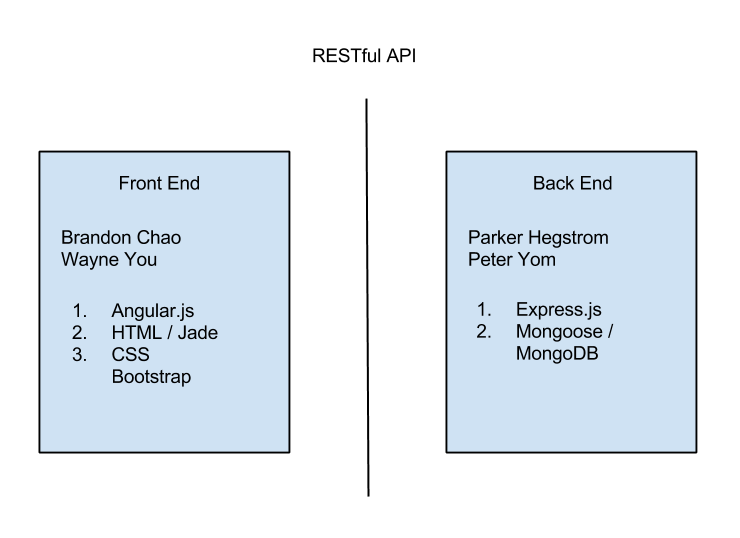
\includegraphics[width=.5\textwidth]{DesignDiagram.png}
\caption{Diagram of our Large Scale Design}
\label{design}
\end{figure}

\noindent Essentially, our back end team provides an exhaustive RESTful API service to our front end. As we received the new requirements for evolution two, the benefits of our modular design came to light as we met to discuss both the refactorings from evolution one that needed to be done and the edits to each modules system design in order to account for the added calendar functionality--event requests and persistent until done events.\\

\noindent The following sections further discuss design choices and implications of those design choices for both our front end and back end teams. \\

\section{Back End Design and Analysis}
\subsection{New Features and Developments}
\subsubsection*{Email Calendars}
This feature was implemented using the \texttt{nodemailer} module that we imported. The back end simply handles the emailing here as the front end actually bundles the proper information (event objects or png) before issuing the request to the server. See front end discussion for more specifics on how the PNG file was created. 
\subsubsection*{En Masse Event Creation}
This feature was pretty simple to execute as we already have a dedicated route to event creation. Hence, given text input, the front end parses the input and issues the needed amount of POST requests to the \texttt{/event} endpoint.
\subsubsection*{Priority Escalation for PUDs}
This feature was a little difficult to implement as previously we had handled priorities by the PUDs index in the users array of PUDs. We thought about scrapping this idea and implementing a priority number, but in the end, we didn't want to change previously written functionality. Hence, we continued to use the array index method for priority. To allow for certain PUDs to escalate, we set a \texttt{willEscalate} property in the database. Using the \texttt{setInterval()} function provided by node, the server checked every day which PUDs need to be escalated, running the escalation algorithm if needed.

\subsubsection*{Preference Sign Ups}
Preference sign ups required the most edits to our pre-existing code in the back end. Specifically, we had to add additional properties to the database model for the Slot Sign Up as well as change the slot sign up creation route (POST to \texttt{/ssu}). Before, this route would finalize the sign up and remove the chosen time block from the available free blocks. Now, we've implemented extra functionality into the async.js waterfall array in the ssu creation process and added a check in the PUT request to the \texttt{/signup/:ssuId} endpoint.\\~\\
The flow for the slot sign up is now this: either the SSU is normal so slots are immediately assigned to a user or the SSU is preference based in which we store the preferred time slots for each user. This information is stored in the \texttt{SlotSignUp.preferences} property of the model. This \texttt{preferences} structure holds the preferences for each user and is ultimately the data used to actually assign the slots at the SSU's deadline.\\~\\
The deadline was repeatedly checked using Node's built-in \texttt{setInterval()} function which was discussed in the previous sub section. \\~\\
Finally, we implemented a simple greedy algorithm to assign the slots to the various invitees. Although this might not produce the optimal assignment in the given matching problem, we felt this was ok due to the fact that the SSU creator would ultimately be able to manually change the assignments before finalizing. This is not the most ideal solution, but in an effort to present a functioning application, we took the hit on scope, something we would continue to expand upon in future developments. See section Future Work for more discussion on this. 


\subsection{Benefits of Our Previous Design}
The major and most noticeable benefit from our previous design was how re-usable it was. From the beginning, we treated the back end of our application as an exposed services API, providing a set of methods that virtually any front end could use. This re-usability came about because we continued to write short and single purpose methods for every service. And on a broader sense, all of our ``routes" were written to complete a single task---create an event, delete a user, send an email, etc. So, for example, when faced with text parsing, all that needed to be done was the actual parsing of the text, because once the data was gathered, it was just a matter of looping through and initiating a POST request to the \texttt{/event} end point for each event. \\~\\
The re-usability came about from our file organization as well. In the third evolution, we began to increase our use of Mongoose.js ``schema" methods (think \texttt{public} java class methods). This allowed us to treat our database models effectively as java classes. Many of our route files might need to convert user ids to user emails, and because of schema methods, we were easily able to make that functionality visible to any file that needed it by using javascript's \texttt{require()} method.

\subsection{Drawbacks of Our Previous Design}
The most time consuming feature was the preference based sign up. Why? Well we discussed that this type of feature---one that modifies pre-existing functionality---was the hardest, but the main reason for its difficulty came about because we made too many assumptions when designing the \texttt{SlotSignUp} model.\\~\\
Before, we had pretty rigid process for handling the slot sign up creation that used async.js \texttt{waterfall()} method. Now, though, certain parts of that async waterfall did not need to be called or additional asynchronous functions needed to be added to the function array. These additions or omittances changed the dependencies between each individual function in the waterfall function array. The required changes were great in number and therefore so were the errors. \\~\\
In addition to specific design pitfalls, another more general problem arose: our file sizes were becoming very large and difficult to follow. As we added more features to pre-existing code, it became apparent that in some files we had just continued to populate the files without giving thought to potentially extracting the code out into a new file---the \texttt{SlotSignUpRoute.js} is almost 500 lines long. I think the solution here is to recognize this earlier and spend more time on discussion of new feature integration rather than just attempting to cram in the new features all into pre-existing architecture. 

\subsection{Future Developments}
For the most part, we on the back-end feel proud of our work and the functionality our application provides. With that being said, there are a couple of things we would continue to develop if we were to get this application customer ready.\\~\\
First, we would spend more optimizing the preference based sign up algorithm. As stated in a previous section, our algorithm is simple and greedy. This works, but does not provide the optimal solution every time it is ran. Ideally we would construct the problem using a bipartite graph (invitees are one type of node, and slots are the other type with edges representing preferences being weighted by preference). If we were able to implement this structure, we could run a simple maximal perfect matching algorithm which would give the optimal assignment.\\~\\
Lastly, we would like to make our application more robust in dealing with errors and form formatting. Currently, no checking is done to see whether or not the user entered in a correct email for example. These aspects of an application are what make it ready for market and would be a must if we were to push this calendar into production.\\~\\

\section{Front End Design and Analysis}

\subsection{New Features and Developments}

\subsubsection{PUD Events}

The extra features to PUD events including an expiry time and priority escalation were handled on the front-end by simply adding fields to the PUD creation form and sending this data to the back-end. Both of these features  took front-end input but the functionality was handled separately in the back-end.

\subsubsection{Preference-based Sign Up}
{\color{red} WAYNE TODO }

\subsubsection{En Masse Event Creation}

We implemented en masse event creation using simple text parsing. Since we have the user input the event with a Name, Description, Start Time, and End Time on separate lines, we simply split the input string based on the new line tokens and create separate events for each series of 4 lines of text.

\subsubsection{Schedule by Email}
Our front-end implementation of this feature was fairly easy. For text schedule, we simply parse through all of the events within the current display frame and send them to the back-end. For image schedule, we take a screenshot of the calendar in the current display using Javascript's html2canvas() function and send it to the back-end to email.

\subsection{Benefits of Our Previous Design}

The implementation of the features in this evolution were fairly straightforward due to our design coming into it. Many of the features seemed to be more back-end oriented which also made our lives a lot easier in this evolution. The only completely new feature was getting the schedule by email, which was a matter of parsing through our list of events we already store for text-based, and used a Javascript function to accomplish the image-based one. Even mass event creation was not hard to create due to the way our events were being created in the past. We merely had a for each loop to create an object with the data for each event we parsed through, and then called our previous event creation route on each event. We really saw the benefits of a flexible design coming into this evolution based on the requested features which allowed us to complete this evolution quickly.

\subsection{Drawbacks of Our Previous Design}

{\color{red} WAYNE TODO }

\section{Individual Portion}
\subsection*{Parker}

\begin{enumerate} [a)]
\item {\bf Designing System Components}
\begin{enumerate} [$\cdot$]
\item I designed the system component that handled the auto PUD creation for all invitees. This required a variable number of asynchronous functions to be executed back to back. More specifically, it was dependent on the number of invitees to the sign up event. To accomplish this in an efficient manner, I created a function that created an array of functions. (see functions \texttt{createWaterfallArray()} and \texttt{createFunctionInArray()} in the file \texttt{SlotSignUpRoutes.js}). In short, I bundled all of the PUD creation code for one user into a variable and created one for each invitee. Async.js executes the array of functions. The benefit from designing the component in this way was to simplify the code and make it more readable. Without this array of functions, there would have been very deep callback hells. The design also allowed us to continue to make use of pre-written libraries that helped with javascript's asynchronous nature, minimizing the amount of code we had to write in the end.
\end{enumerate}
\item  {\bf Designing and Conducting Experiments}
\begin{enumerate} [$\cdot$]
\item For the auto pud creation feature in preference based sign ups, we had to perform a number of asynchronous operations based on an input size (number of invitees). To do this, I had to create an array of functions which was only made possible by the fact that javascript uses first-class functions. To test this function array creation, I started writing simple examples. I would then loop through the array of functions, executing each and making sure they executed correctly. The next steps were to gradually turn my simple examples into ones that performed the functionality required by the feature. This iterative, experimental process proved to be extremely time consuming as it allowed me to fully understand the inner workings of some of the async.js library functions.
\end{enumerate}	
\item  {\bf Analyzing and Interpreting Data}
\begin{enumerate} [$\cdot$]
\item One use of first class functions is the callback, a way that javascript handles asynchronous functions. I wrote my own asynchronous function that utilized a callback exit. Unfortunately this function produced an error I had never seen before, one that dealt with HTTP protocols. Specifically the response header was being set after the response had been sent. Confusing! However, I was able to read the stack trace in the console, pinpoint the location of the error, and deduce the type of error. With the error type and location, I was able to eventually fix the bug by reading internet forums and Express.js API pages.
\end{enumerate}
\item {\bf Dealing with Realistic Constraints}
\begin{enumerate} [$\cdot$]
\item A realistic constraint I encountered was my lack of knowledge for how javascript treated functions. To get around this, I simply had to do a lot of side reading on my own. I watched video tutorials and read online forums like stack exchange. 
\end{enumerate}
\item  {\bf Teamwork and Team Member Interaction}
\begin{enumerate} [$\cdot$]
\item For this evolution, I would say we worked much more independently than in previous evolutions. Our schedules did not permit too many in person meetings. This turned out to be completely fine as, apart from some small changes, our group was able to function very efficiently in this manner. It was a learning experience for the better!
\end{enumerate}
\end{enumerate}

\subsection*{Peter}

\begin{enumerate} [a)]
\item  {\bf Designing and Conducting Experiments}
\begin{enumerate} [$\cdot$]
\item 
\end{enumerate}
\item  {\bf Analyzing and Interpreting Data}
\begin{enumerate} [$\cdot$]
\item 
\end{enumerate}
\item {\bf Designing System Components}
\begin{enumerate} [$\cdot$]
\item 
\end{enumerate}
\item {\bf Dealing with Realistic Constraints}
\begin{enumerate} [$\cdot$]
\item 
\end{enumerate}
\item  {\bf Teamwork and Team Member Interaction}
\begin{enumerate} [$\cdot$]
\item 
\end{enumerate}
\end{enumerate}

\subsection*{Brandon}

\begin{enumerate} [a)]
\item  {\bf Designing and Conducting Experiments}
\begin{enumerate} [$\cdot$]
\item Wayne initially implemented getting the schedule in image format by using the html2canvas() function to take screenshots of the page based on the DOM. However, the limitation to this is that we can only get the image of the time range that is currently being displayed. As such, I experimented with taking and storing images of multiple weeks/months and sending them all at once to the user. I did this by changing the view of the calendar (and the DOM) and taking a screenshot at each requested month using the same function. However, this didn't seem to work because I was not able to change the view of the calendar without it rerendering on the front-end which caused it to keep changing the display. Also, I was having trouble sending an array of image data URLs to the back-end to represent each week or month that was requested. Because of these issues, we ultimately decided to limit the functionality of getting the schedule in image format to only send the current time frame to the user.
\end{enumerate}
\item  {\bf Analyzing and Interpreting Data}
\begin{enumerate} [$\cdot$]
\item When I was implementing reordering of Slot Sign Ups to allow the owner to decide slots based on their preference, I ran into the issue of the slots not updating their reorder in real-time. However, when I printed them out after grabbing them from the back-end, they were in the expected order. This led me to believe that whichever scope variable we were using to display them on the front-end wasn't being updated correctly. I confirmed this by printing out the array of objects for the ordered slots from the Angular code and saw that they were indeed incorrect. This was solved by updating the scope variable upon successful execution of the HTTP PUT. We have run into numerous similar issues in the past which made debugging this fairly easy. However, if I had time to continue working on the calendar, one thing I would refactor is cleaning up our controllers and which scope the variables were placed in by creating a better hierarchy of controllers.
\end{enumerate}
\item {\bf Designing System Components}
\begin{enumerate} [$\cdot$]
\item One component we had to design was the detail display for preference-based signups. We decided that we wanted the owner to view the Slot Sign Up details modal unless all requested users have signed up for slots already and it was time for the owner to resolve the conflicts. In that case, we bring the owner to the Slot Sign Up resolution modal. After resolution, subsequent clicks of that particular slot sign up will once again take the user to the details modal. We achieved this by maintaining two flags stored within the scope for the particular slot sign up. We maintain one flag to check if the preferences for slot sign ups are complete, as in all requested users have signed up, and one flag to check if the preferences for slot sign ups are final, as in the owner has resolved any conflicts. Each time the slot sign up is clicked, we check these flags to determine which modal to display. This currently does not allow the owner to edit a slot resolution after they submit it, but adding this would simply require a button that would toggle the final flag for this particular slot sign up which would allow the owner to make changes after submission. 
\end{enumerate}
\item {\bf Dealing with Realistic Constraints}
\begin{enumerate} [$\cdot$]
\item One realistic constraint that we had to consider was when we were implementing the graphical schedule by email. We did this by taking a screenshot of the current time frame of the calendar. While this wasn't very difficult, the nature of the html2canvas() Javascript function we used to do this made it difficult to get a graphical display of calendars that you were not currently on. For example, to get a graphical schedule of the next month, you would need to manually click next month and then send the image file. We experimented with using various other functions to achieve this, but the html2canvas() function provided the easiest implementation.
\end{enumerate}
\item  {\bf Teamwork and Team Member Interaction}
\begin{enumerate} [$\cdot$]
\item We made an effort to start implementing the features of this evolution a lot earlier this time. As a result, by the night before it was due, we had a lot fewer pressing errors to resolve last minute. I felt that teamwork and team member interaction went a lot more smoothly because of this and because we met up in person earlier to work out bugs.
\end{enumerate}
\end{enumerate}
\subsection*{Wayne}

\begin{enumerate} [a)]
\item  {\bf Designing and Conducting Experiments}
\begin{enumerate} [$\cdot$]
\item 
\end{enumerate}
\item  {\bf Analyzing and Interpreting Data}
\begin{enumerate} [$\cdot$]
\item  
\end{enumerate}
\item {\bf Designing System Components}
\begin{enumerate} [$\cdot$]
\item 
\end{enumerate}
\item {\bf Dealing with Realistic Constraints}
\begin{enumerate} [$\cdot$]
\item 
\end{enumerate}
\item  {\bf Teamwork and Team Member Interaction}
\begin{enumerate} [$\cdot$]
\item 
\end{enumerate}
\end{enumerate}

%\keywords{Cremona map \and Newton complementary dual \and monoid \and Cohen--Macaulay}

%\vspace{0.2in}




%\begin{align}
%e^{j\theta} = cos(\theta) + jsin(\theta)
%\end{align}

%\begin{figure}[h]
%\begin{center}
%\epsfig{file=StatPlot.eps, width=5in}
%\caption{\label{boxplot} Box plot of the survey data}
%\end{center}
%\end{figure}


%\begin{figure}[h]
%\begin{center}
%\epsfig{file=histogram.eps, width=4in}
%\caption{\label{histogram} Histogram plot of the survey data}
%\end{center}
%\end{figure}

%\begin{table}[h]
%\begin{center}
%\caption{\label{histotable}Table of frequency values from the Histogram} 
%\begin{tabular}{|c|c|}\hline
%{\bf Type of Engineering} & Frequency \\
%BME & 59 \\
%CEE & 6 \\
%ME & 3 \\
%ECE & 10 \\
%Undecided & 1 \\ \hline
%\end{tabular} \\~\\
%\end{center}
%\end{table}

%\begin{figure}[htb]
%\centering
%\includegraphics[width=1.3\textwidth]{Screenshot.png}
%\caption{Screen shot from StatKey}
%\label{samples}
%\end{figure}


%\appendix
%\section{Codes}
%\subsection{MakeGraph.m}
%\listinginput[1]{1}{MakeGraph.txt}


% GIVES TWO TABLES BY EACHOTHER
%\begin{table}[h!]
%\begin{minipage}[b]{0.45\linewidth}\centering
%\caption{\label{ecoli3}Using {\tt ecoli\_edit\_120481.txt}} 
%\begin{tabular}{|c|c|c|}
%\hline
%1 & 1 & 1 \\
%\hline
%\end{tabular}
%\end{minipage}
%\hspace{0.5cm}
%\begin{minipage}[b]{0.45\linewidth}
%\centering
%\caption{\label{ecoli4}Using {\tt ecoli\_edit\_3947161.txt}} 
%\begin{tabular}{|c|c|c|}
%\hline
%1 & 1 & 1 \\
%\hline
%\end{tabular}
%\end{minipage}
%\end{table}

\end{document}
% end of file template.tex
